\documentclass[11pt, a4paper]{article}
\usepackage{pdfpages}
\usepackage{parallel}
\usepackage[T2A]{fontenc}
\usepackage{ucs}
\usepackage[utf8x]{inputenc}
\usepackage[polish,english,russian]{babel}
\usepackage{hyperref}
\usepackage{rotating}
\usepackage[inner=2cm,top=1.8cm,outer=2cm,bottom=2.3cm,nohead]{geometry}
\usepackage{listings}
\usepackage{graphicx}
\usepackage{wrapfig}
\usepackage{longtable}
\usepackage{indentfirst}
\usepackage{array}
\usepackage{tikzsymbols}
\usepackage{soul}
\usepackage[ruled,vlined]{algorithm2e}
%\counterwithout{figure}{section} 

\usepackage{url}
\makeatletter
\g@addto@macro{\UrlBreaks}{\UrlOrds}
\makeatother

\newcolumntype{P}[1]{>{\raggedright\arraybackslash}p{#1}}
\frenchspacing
\usepackage{fixltx2e} %text sub- and superscripts
\usepackage{icomma} % коскі ў матэматычным рэжыме
\PreloadUnicodePage{4}

\newcommand{\longpage}{\enlargethispage{\baselineskip}}
\newcommand{\shortpage}{\enlargethispage{-\baselineskip}}

\def\switchlang#1{\expandafter\csname switchlang#1\endcsname}
\def\switchlangbe{
\let\saverefname=\refname%
\def\refname{Літаратура}%
\def\figurename{Іл.}%
}
\def\switchlangen{
\let\saverefname=\refname%
\def\refname{References}%
\def\figurename{Fig.}%
}
\def\switchlangru{
\let\saverefname=\refname%
\let\savefigurename=\figurename%
\def\refname{Литература}%
\def\figurename{Рис.}%
}

\hyphenation{admi-ni-stra-tive}
\hyphenation{ex-pe-ri-ence}
\hyphenation{fle-xi-bi-li-ty}
\hyphenation{Py-thon}
\hyphenation{ma-the-ma-ti-cal}
\hyphenation{re-ported}
\hyphenation{imp-le-menta-tions}
\hyphenation{pro-vides}
\hyphenation{en-gi-neering}
\hyphenation{com-pa-ti-bi-li-ty}
\hyphenation{im-pos-sible}
\hyphenation{desk-top}
\hyphenation{elec-tro-nic}
\hyphenation{com-pa-ny}
\hyphenation{de-ve-lop-ment}
\hyphenation{de-ve-loping}
\hyphenation{de-ve-lop}
\hyphenation{da-ta-ba-se}
\hyphenation{plat-forms}
\hyphenation{or-ga-ni-za-tion}
\hyphenation{pro-gramming}
\hyphenation{in-stru-ments}
\hyphenation{Li-nux}
\hyphenation{sour-ce}
\hyphenation{en-vi-ron-ment}
\hyphenation{Te-le-pathy}
\hyphenation{Li-nux-ov-ka}
\hyphenation{Open-BSD}
\hyphenation{Free-BSD}
\hyphenation{men-ti-on-ed}
\hyphenation{app-li-ca-tion}

\def\progref!#1!{\texttt{#1}}
\renewcommand{\arraystretch}{2} %Іначай формулы ў матрыцы зліпаюцца з лініямі
\usepackage{array}

\def\interview #1 (#2), #3, #4, #5\par{

\section[#1, #3, #4]{#1 -- #3, #4}
\def\qname{LVEE}
\def\aname{#1}
\def\q ##1\par{{\noindent \bf \qname: ##1 }\par}
\def\a{{\noindent \bf \aname: } \def\qname{L}\def\aname{#2}}
}

\def\interview* #1 (#2), #3, #4, #5\par{

\section*{#1\\{\small\rm #3, #4. #5}}
\ifx\ParallelWhichBox\undefined%
    \addcontentsline{toc}{section}{#1, #3, #4}%
\else%
\ifnum\ParallelWhichBox=0%
    \addcontentsline{toc}{section}{#1, #3, #4}%
\fi\fi%

\def\qname{LVEE}
\def\aname{#1}
\def\q ##1\par{{\noindent \bf \qname: ##1 }\par}
\def\a{{\noindent \bf \aname: } \def\qname{L}\def\aname{#2}}
}

\newcommand{\interviewfooter}[1]{
\vskip 1em
\noindent \textit{#1}
}


\begin{document}

\title{1982 "--- Dépraz/Logitech DIGIMOUSE}
\date{}
\maketitle

Конструкция данной мыши, первоначально выпущенной часовой компанией Dubois Depraz SA, была разработана в Андре Гиньяром и профессором Жаном-Даниэлем Никудом из Федеральной политехнической школы Лозанны в Швейцарии в 1977 году. Особенностью разработки были опто-механические энкодеры, значительно улучшавшие оригинальную конструкцию Дугласа Энгельбарта. Однако из-за отсутствия программного обеспечения, поддерживавшего управление мышью, реальное распространение Dépraz Mouse получила после 1982 года, когда Logitech приобрела ее производство у Dubois Depraz SA и выпустила в продажу как первую мышь Logitech, под названием <<P-4 Mouse>>.
Помимо Logitech, Dépraz Mouse производилась для собственных персональных компьютеров Smaky Жана-Даниэля Никуда. Кроме того, Logitech поставляла P4 как OEM-оборудование для компьютеров ряда известных компаний: DEC, Hewlett-Packard, AT\&T, Convergent Technologies. Наиболее распространенным был вариант с ярко-красным корпусом и черными кнопками (рис. \ref{fig:DIGIMOUSEP4Pic}); реже встречаются варианты с бежевым и белым корпусом, а также несколько специальных расцветок, например P4 для компании IDS в синем корпусе с белыми кнопками и Smaky Mouse в голубом корпусе с красными кнопками. 

\begin{figure}[h]
   \centering
    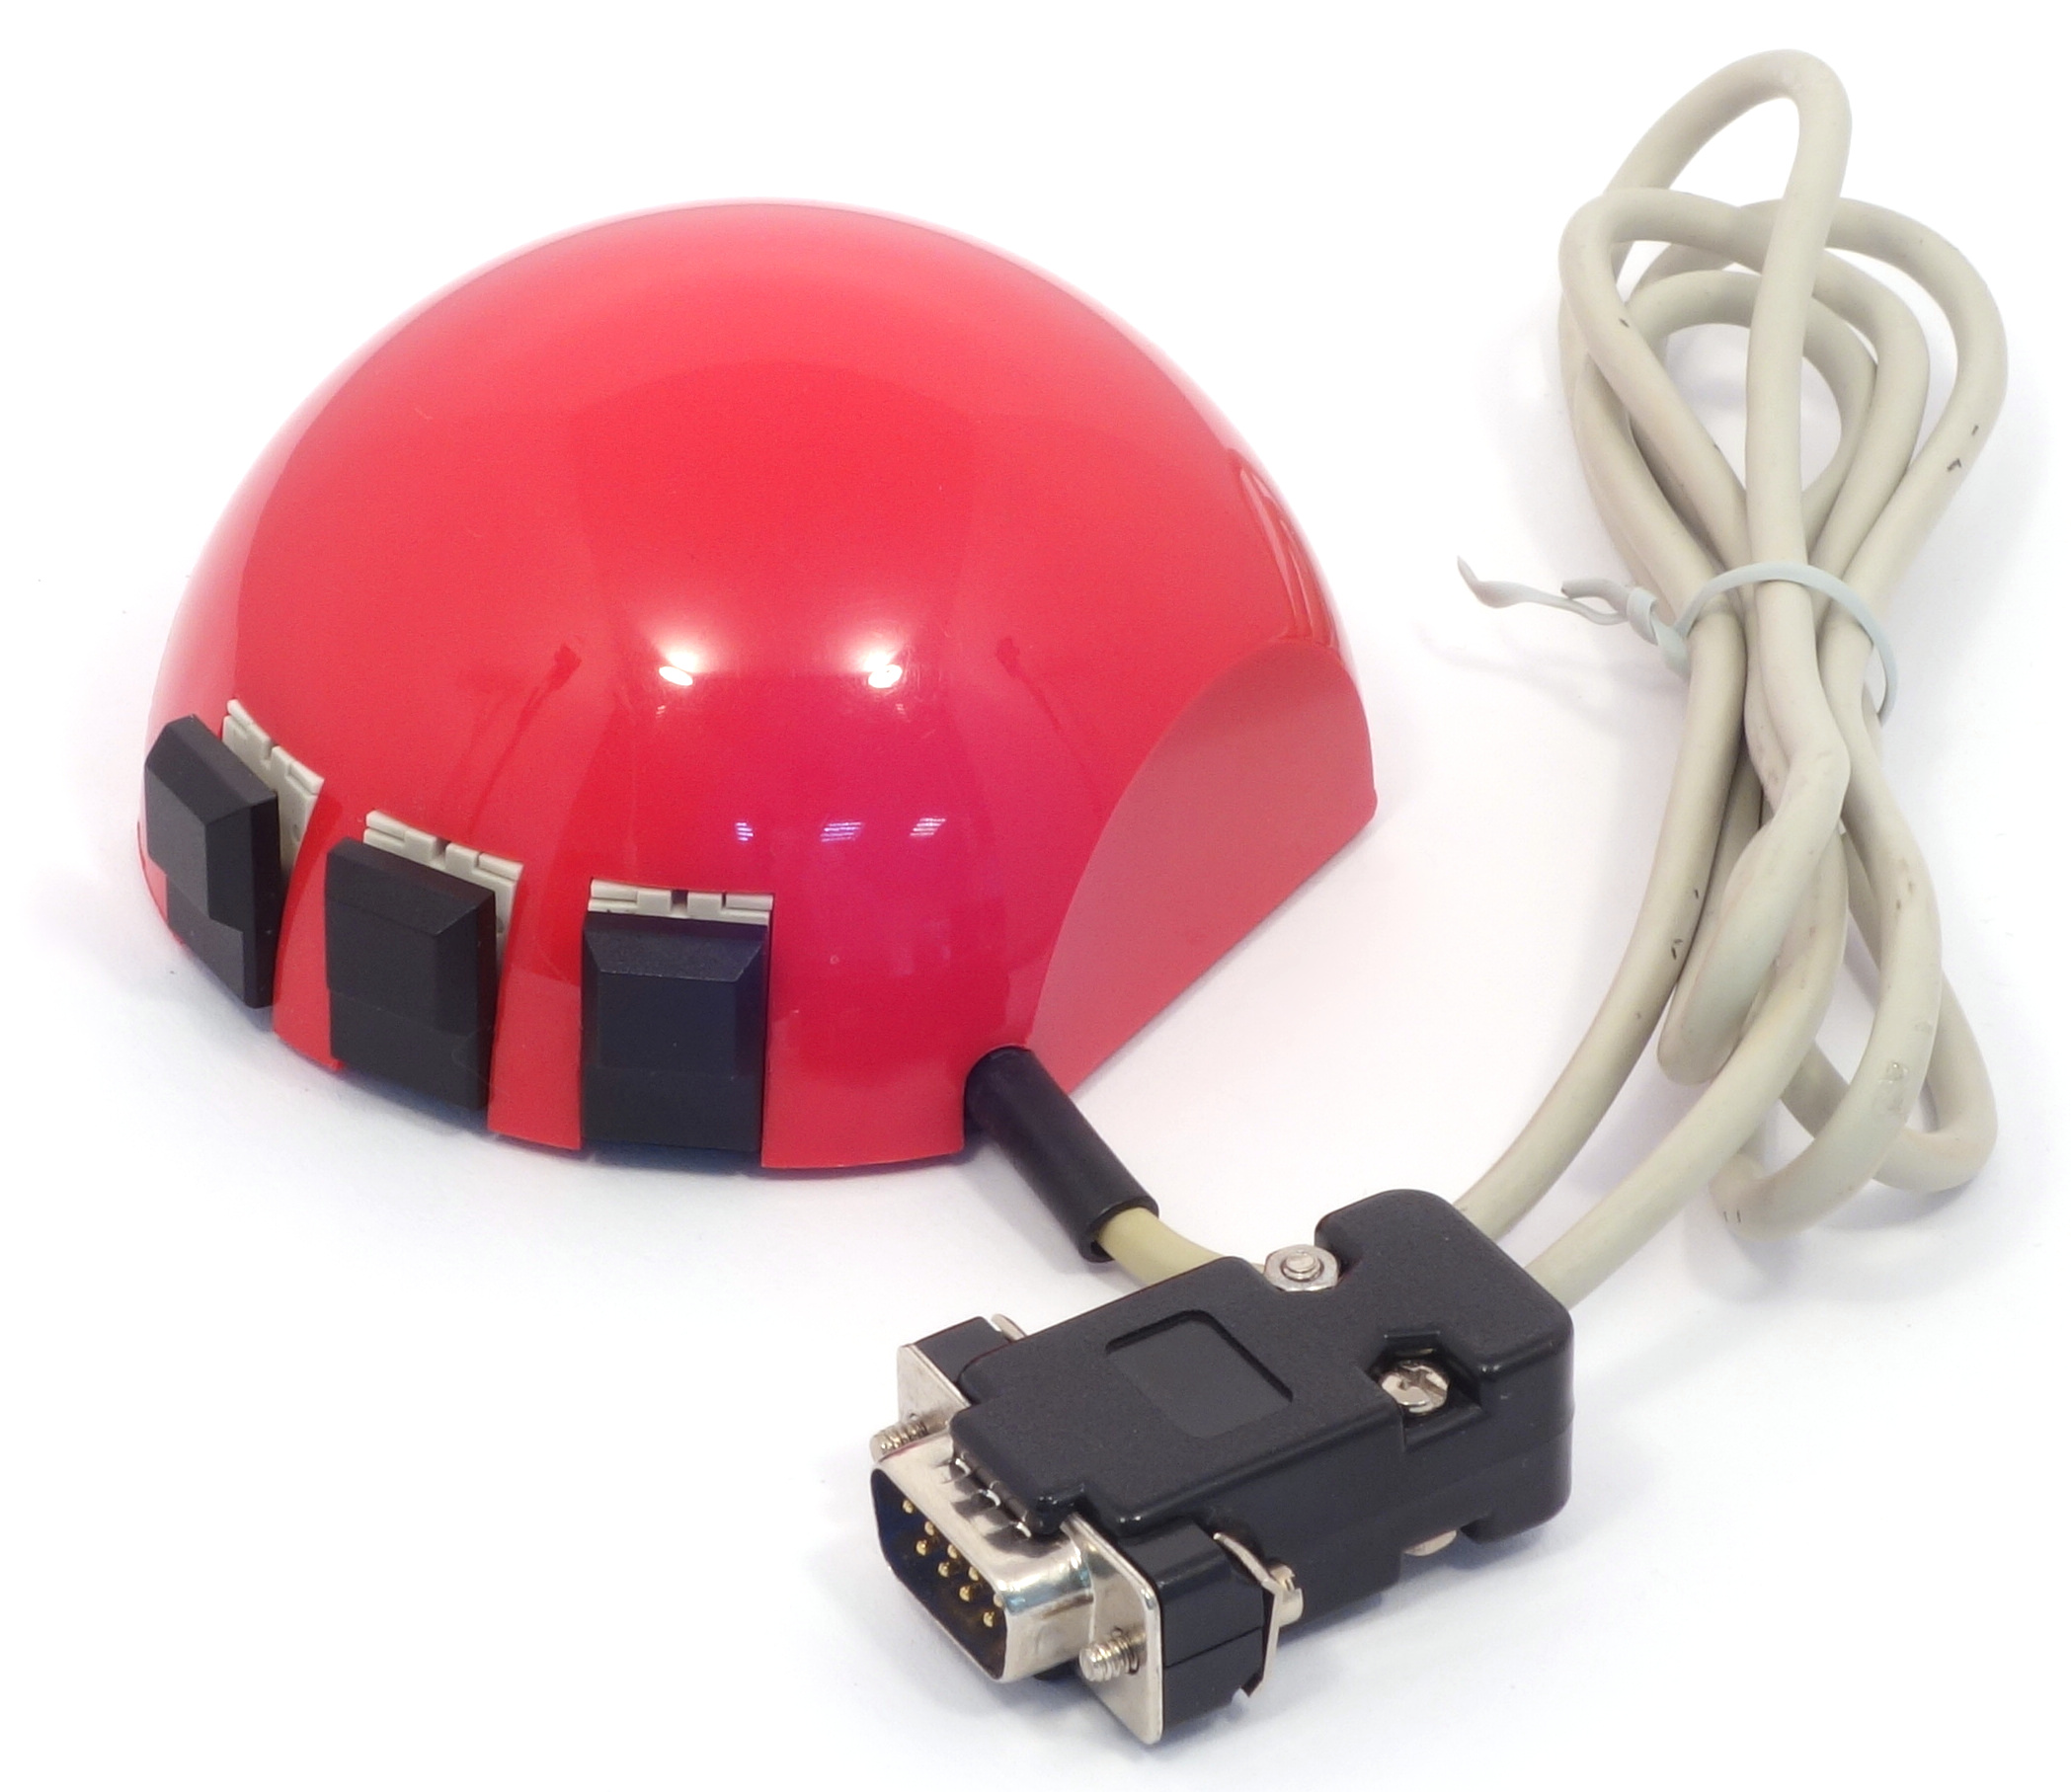
\includegraphics[scale=0.5]{1982_depraz_digimouse/pic_60.jpg}
    \caption{DIGIMOUSE P4, вид спереди}
    \label{fig:DIGIMOUSEP4Pic}
\end{figure}

Одна и та же мышь могла быть брэндирована в разных вариациях как Dépraz Mouse, Logitech P4, DIGIMOUSE 1000 P (рис. \ref{fig:DIGIMOUSEP4TopAndBottom}).

\begin{figure}[h]
    \centering
    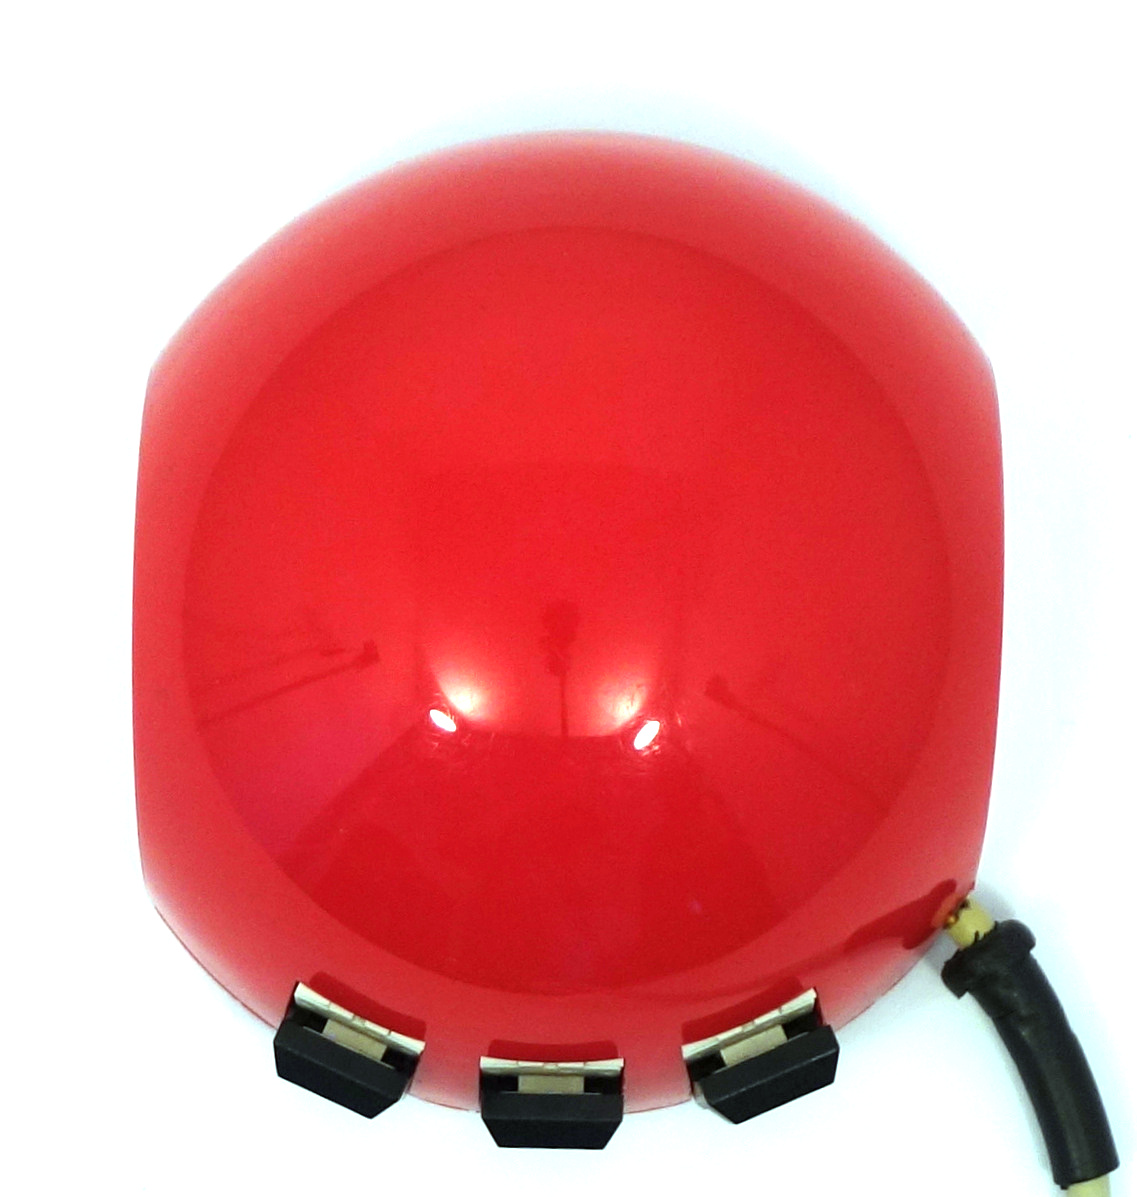
\includegraphics[scale=0.4]{1982_depraz_digimouse/top_60.jpg}
    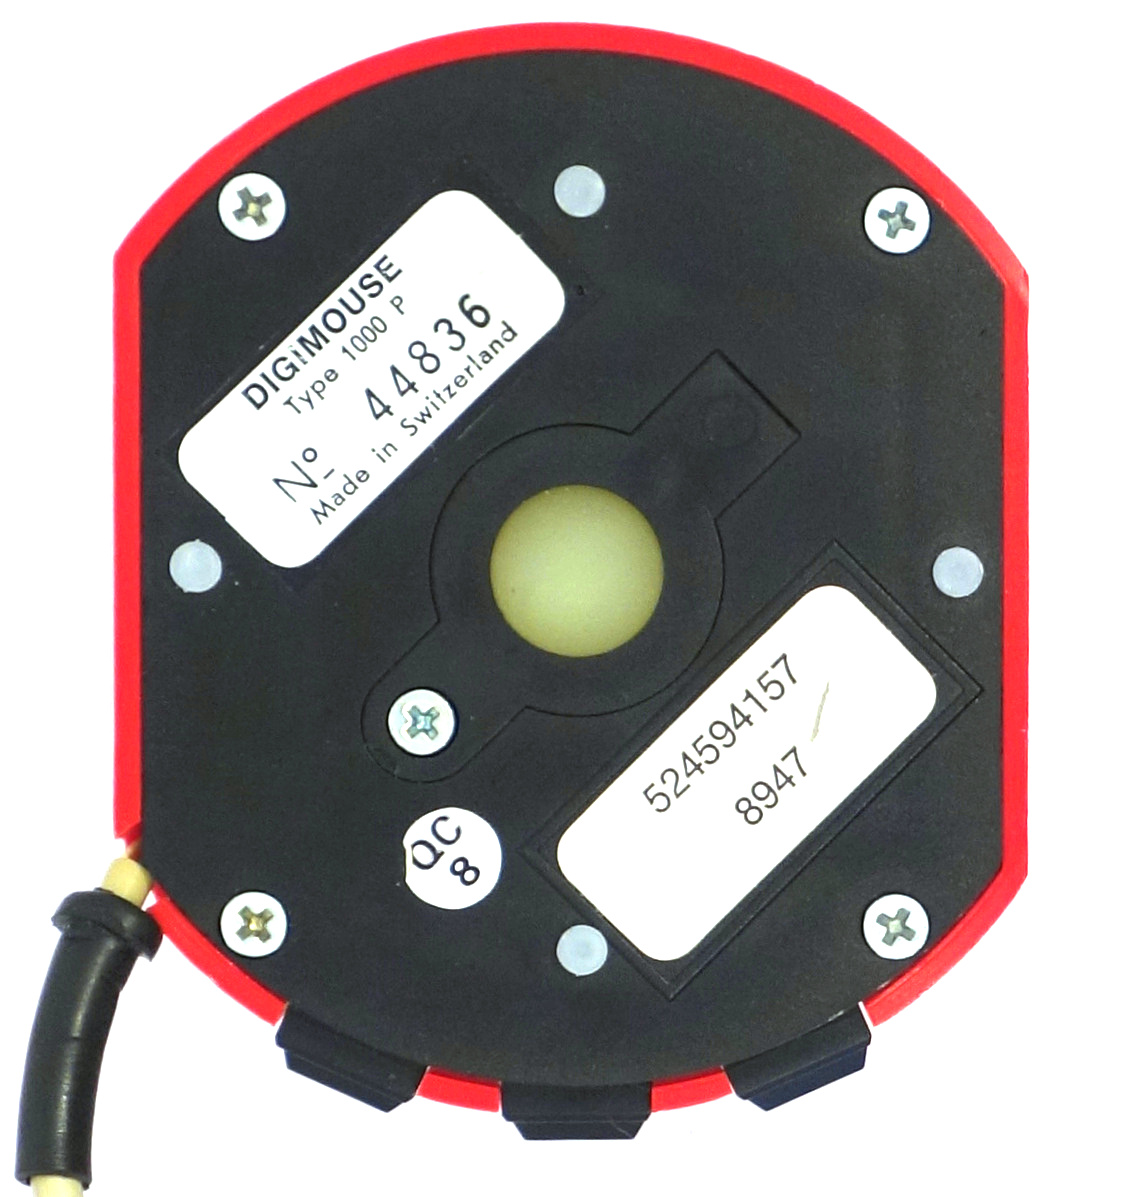
\includegraphics[scale=0.37]{1982_depraz_digimouse/bottom_60.jpg}
    \caption{DIGIMOUSE P4, вид сверху и снизу}
    \label{fig:DIGIMOUSEP4TopAndBottom}
\end{figure}

Мышь имеет размеры, типичные для мышей 1980-х годов (рис. \ref{fig:DIGIMOUSEP4Size}).

\begin{figure}[h]
    \centering
    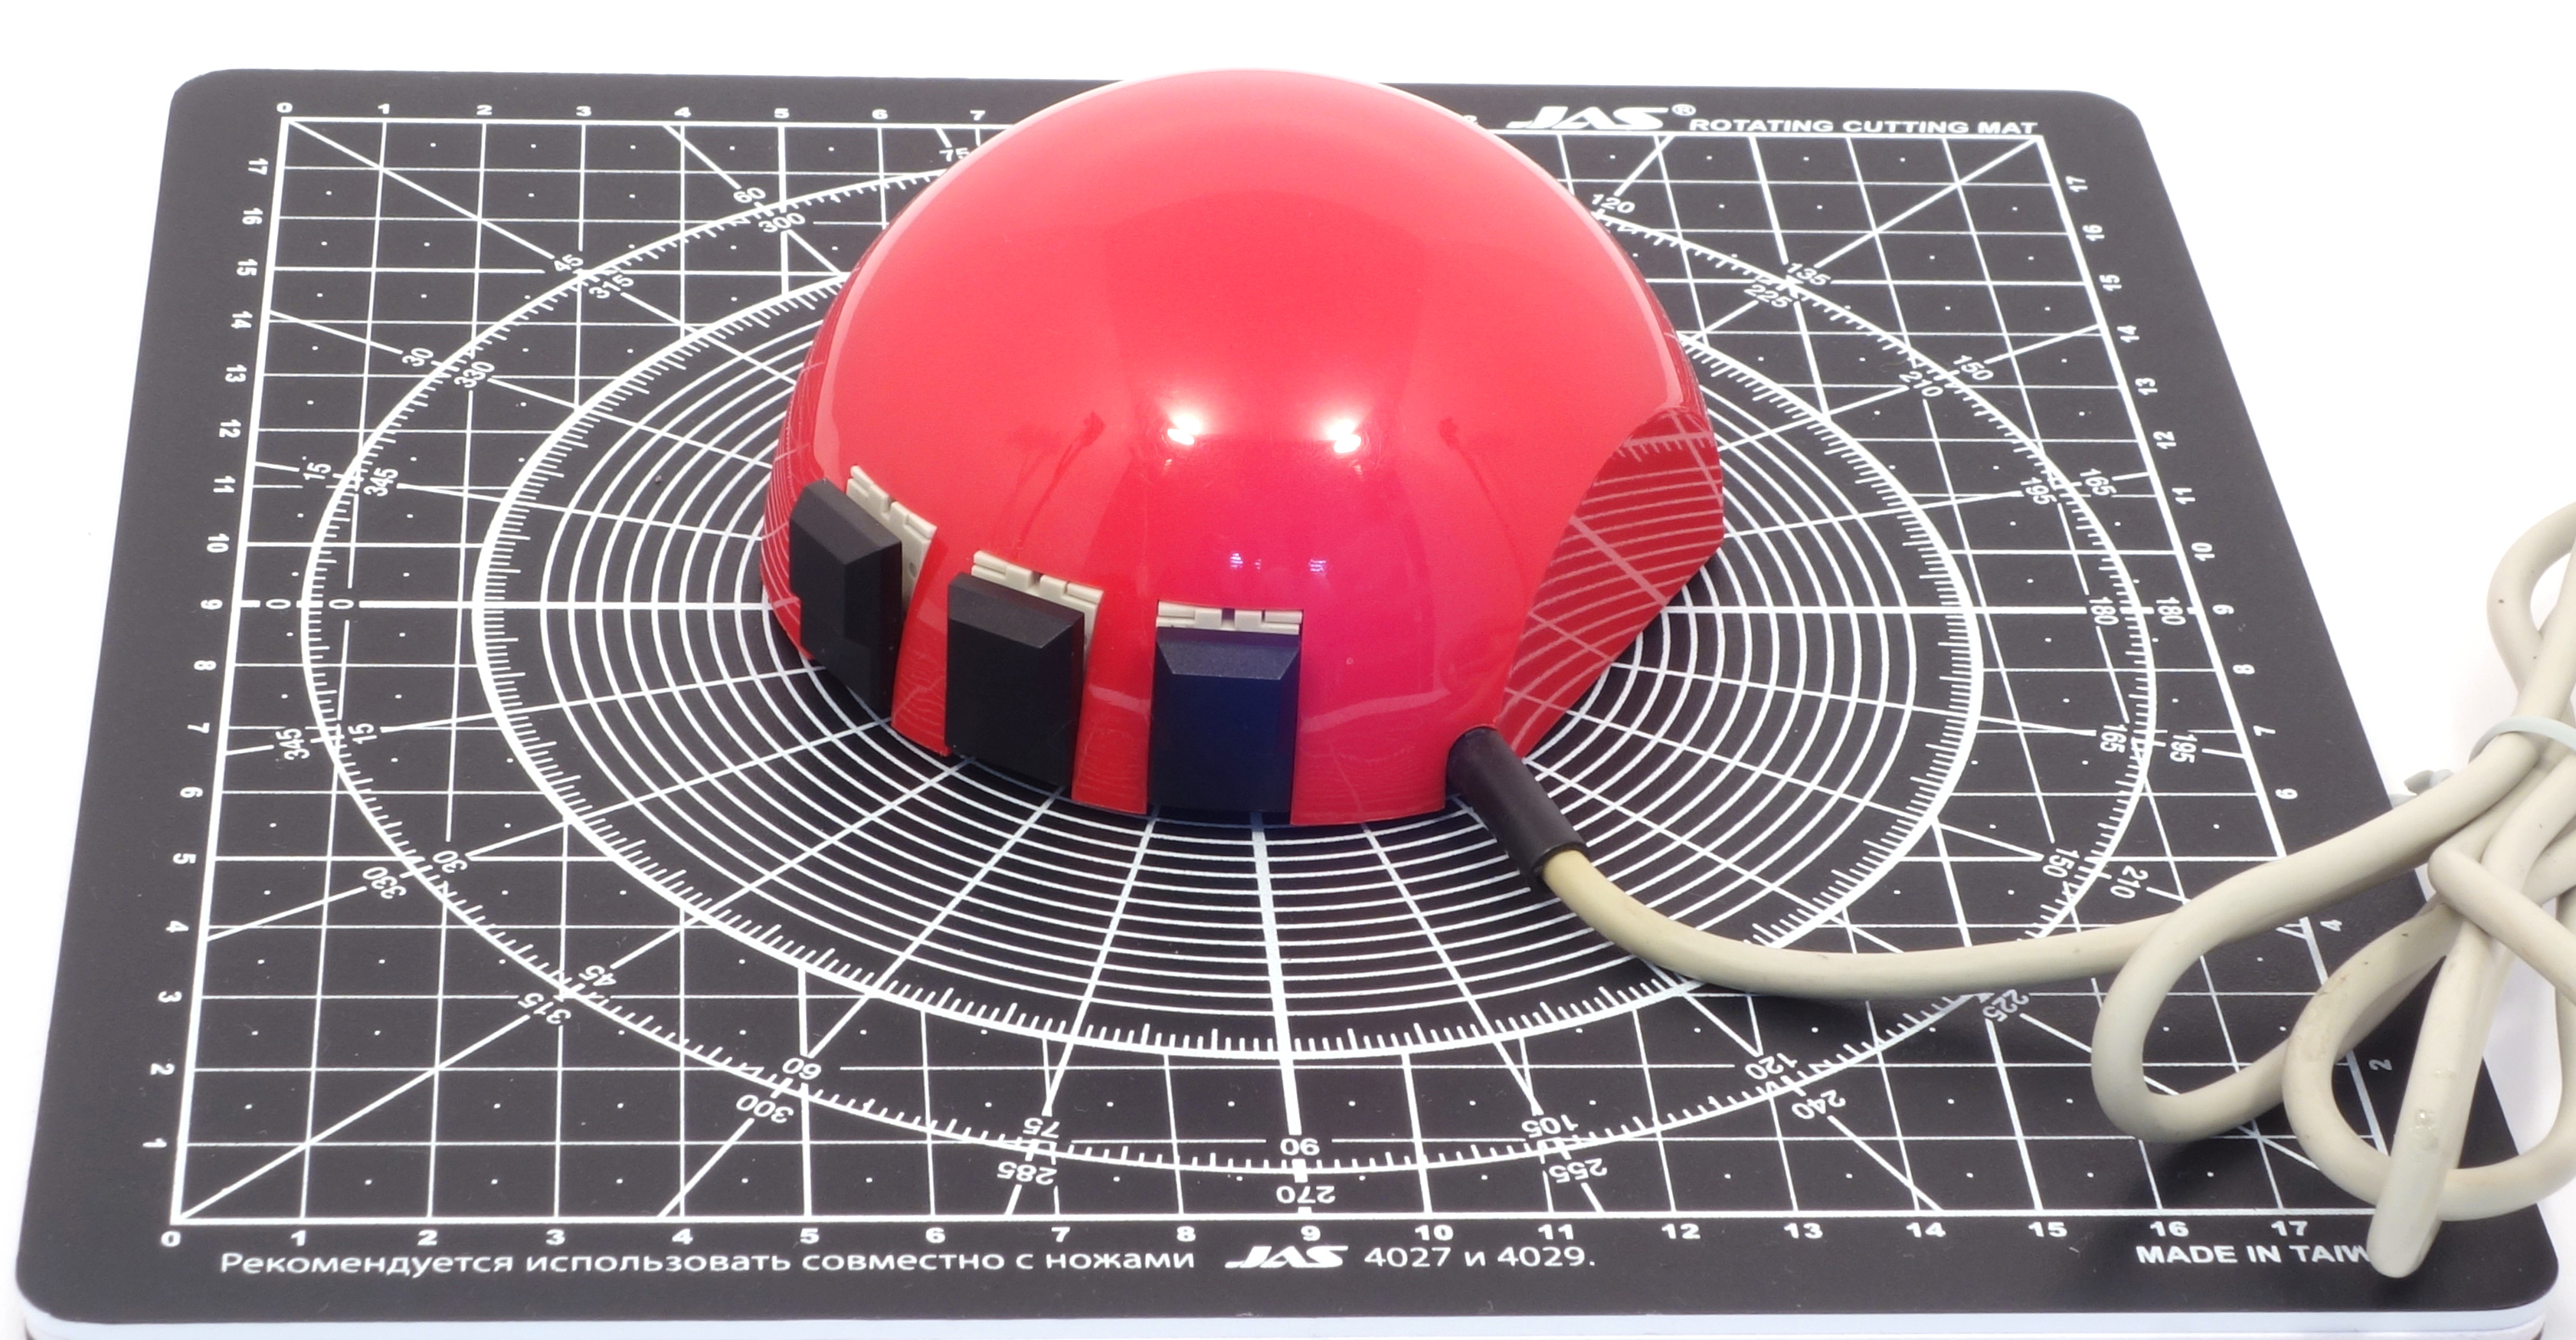
\includegraphics[scale=0.5]{1982_depraz_digimouse/size_30.jpg}
    \caption{DIGIMOUSE P4 на размерном коврике с шагом сетки 1~см}
    \label{fig:DIGIMOUSEP4Size}
\end{figure}

Корпус представляет собой полусферу диаметром 3 ½ дюйма, обрезанную по бокам для удобного захвата большим пальцем и мизинцем. На дальней от пользователя стороне корпуса расположены вертикально три подпружиненные кнопки, обладающие отчетливым щелчком и тактильным откликом на срабатывание \cite{oldmouse}. Из-за расположения кнопок, занимающих всю переднюю стенку корпуса, кабель выведен из корпуса по диагонали. Такая форма получила название <<купола>> и оказалась одной из первых по-настоящему удачных форм корпуса мыши: геометрическая простота сочетается с хорошей эргономичностью, благодаря чему мышь приятно держать в руке (рис. \ref{fig:DIGIMOUSEP4Hand}). Обладатели маленьких ладоней могут легко опереться запястьем на стол или поднять его вверх при необходимости использовать кнопки.

\begin{figure}[h]
    \centering
    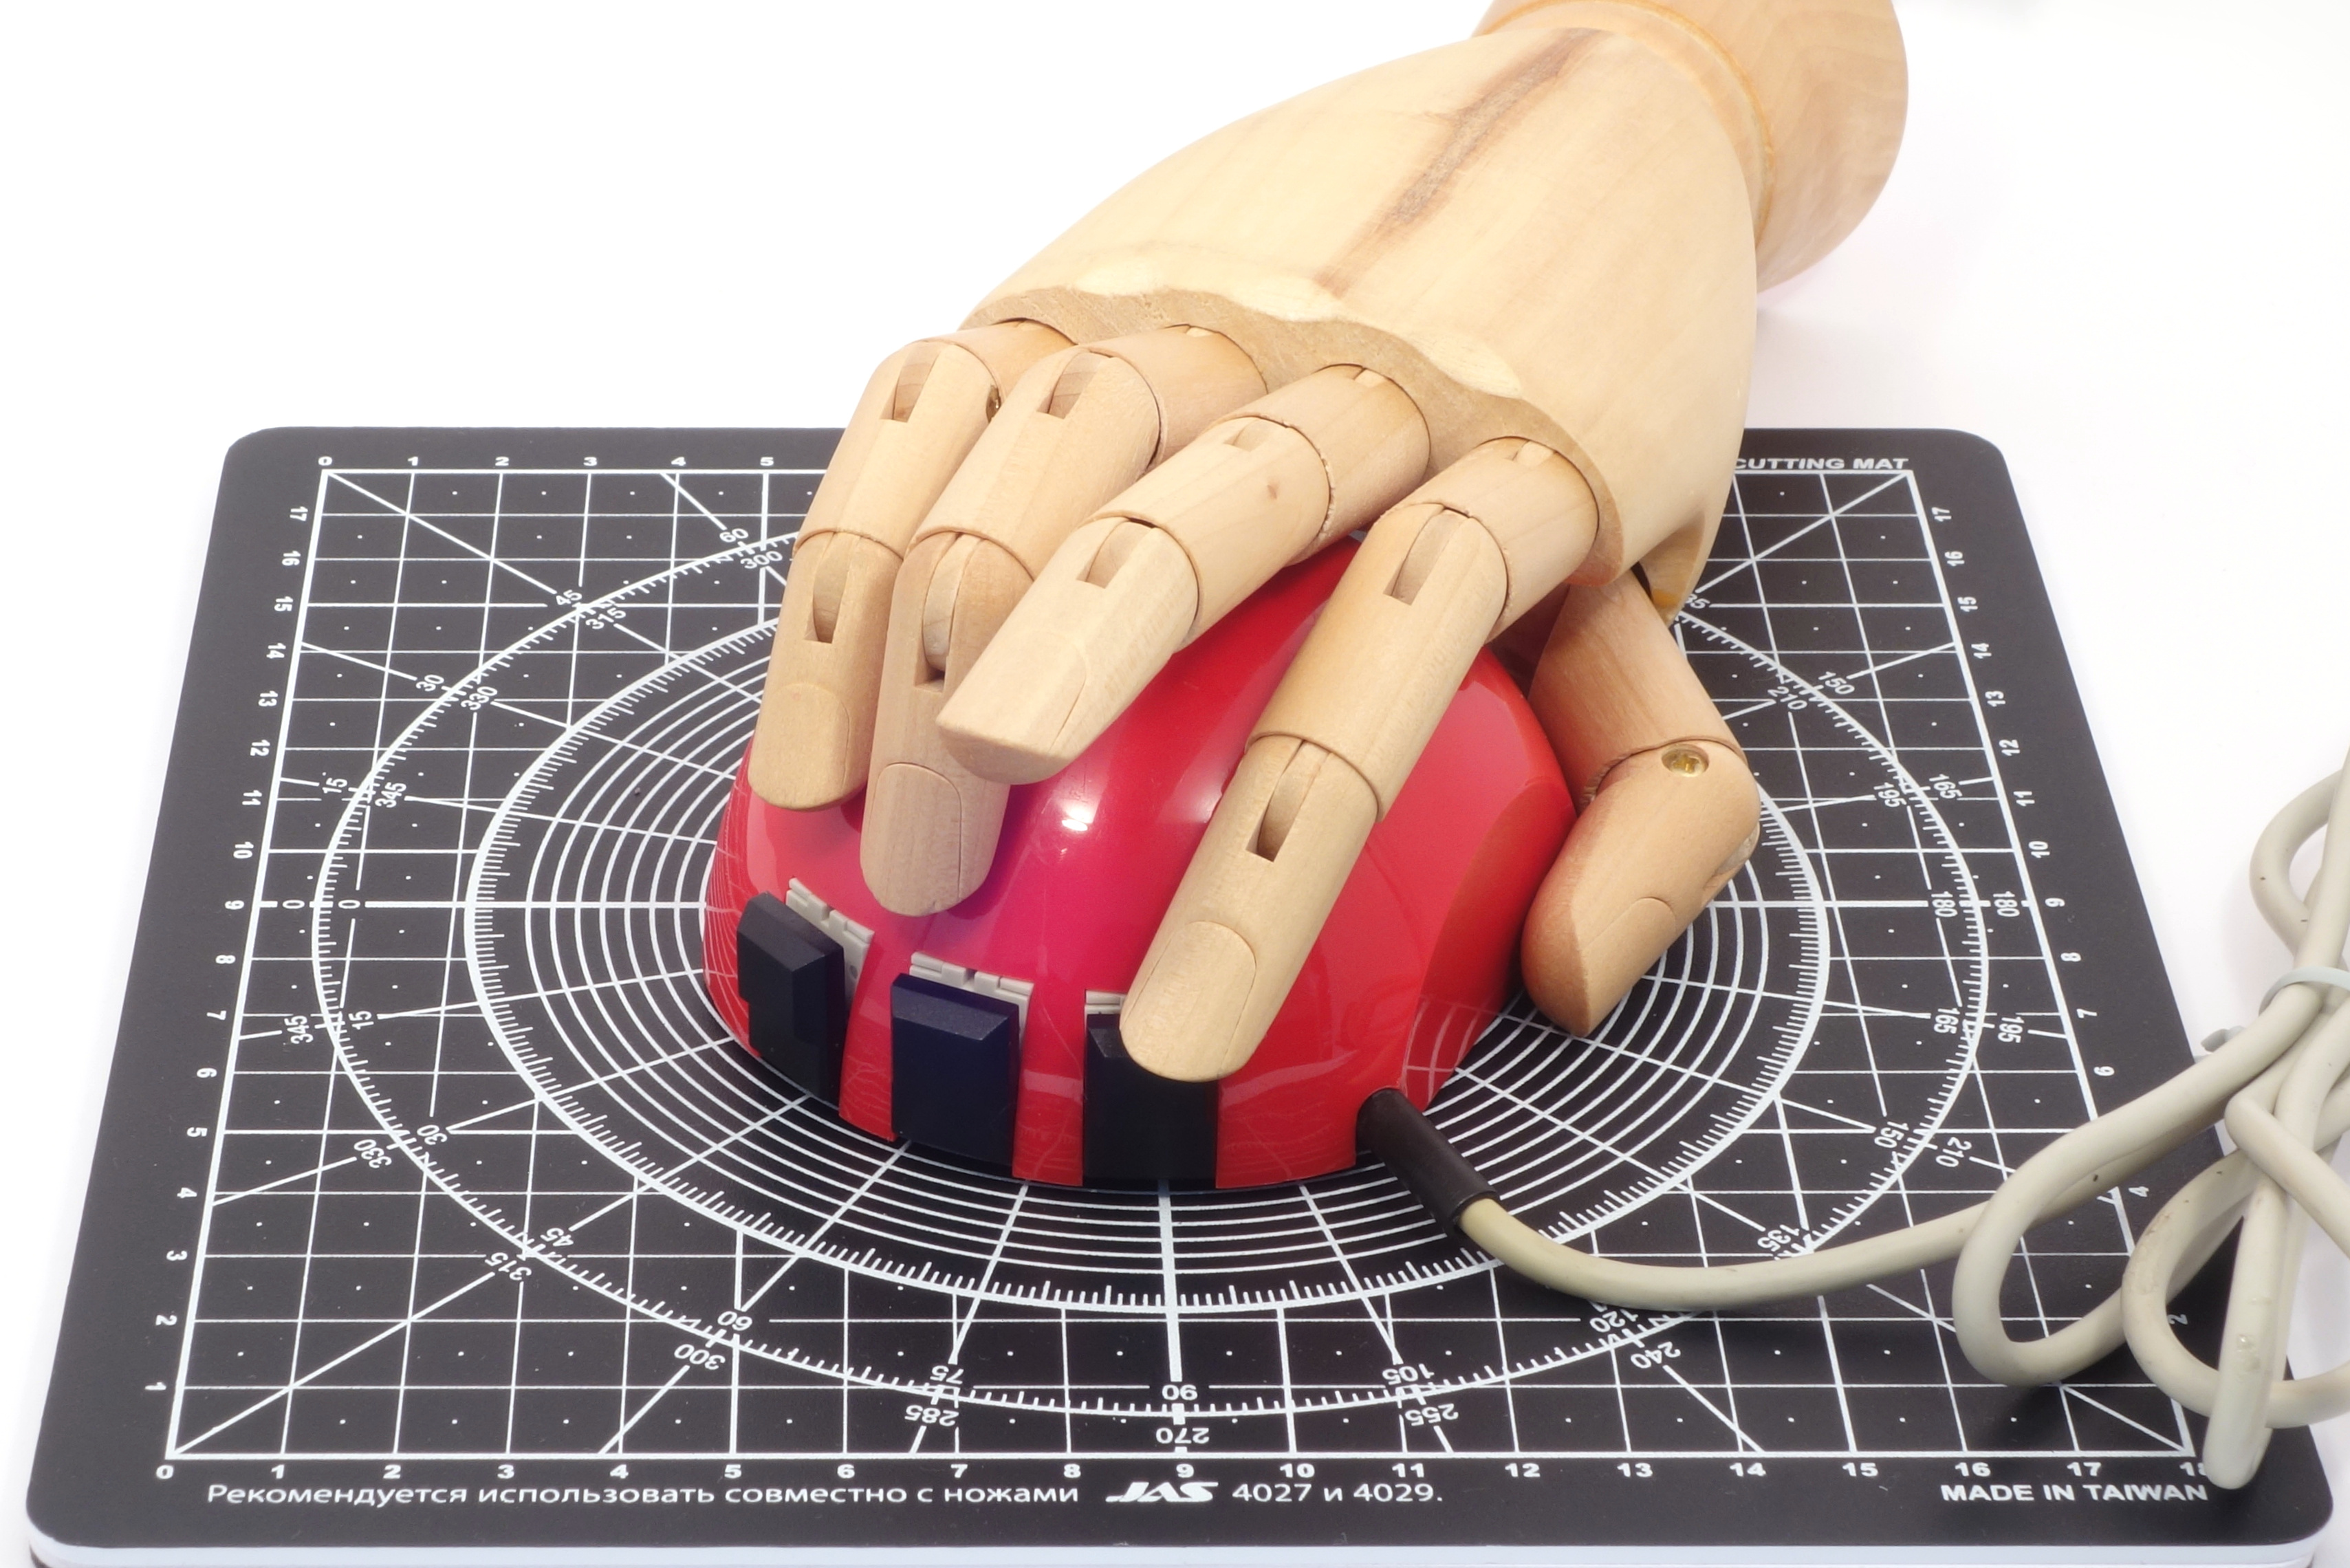
\includegraphics[scale=0.5]{1982_depraz_digimouse/hand_30.jpg}
    \caption{DIGIMOUSE P4 с моделью руки человека}
    \label{fig:DIGIMOUSEP4Hand}
\end{figure}

Мышь имеет разрешение 381 DPI. Начиная с 1984 года, в качестве дополнительного аксессуара P4 могли комплектоваться специальным адаптером-переходником LogiMate \cite{oldmouse}, который позволял подключить мышь не к отдельному адаптеру с шинным интерфейсом, а в разрыв кабеля клавиатуры. При таком подключении перемещение мыши приводило к генерации кодов нажатий клавиш управления курсором: в стандартном режиме разрешение составляло 12 нажатий клавиш на дюйм по горизонтали и 6 нажатий по вертикали, что было рассчитано на работу в текстовом режиме 80x25 символов. В обзоре PC Magazine отмечается, что использование мыши в стандартном режиме позволяло перемещать курсор в текстовом редакторе в семь раз быстрее, чем соответствующие клавиши на клавиатуре (однако требовалось привыкнуть к тому, что в результате небольшого промаха пользователя за крайней правой позицией курсор текстового редактора неизменно перескакивал на левую позицию следующей строки). По очевидным причинам для использования мыши не требовался драйвер; однако его применение давало возможность дополнительных настроек "--- например, позволяло выставлять разрешение переходника LogiMate в диапазоне 1--100 нажатий на дюйм, а также переназначить действие клавиш мыши (по-умолчанию генерировались коды клавиш F8, F9 и F10) \cite{DIGIMOUSE}.

 \begin{figure}[h]
    \centering
    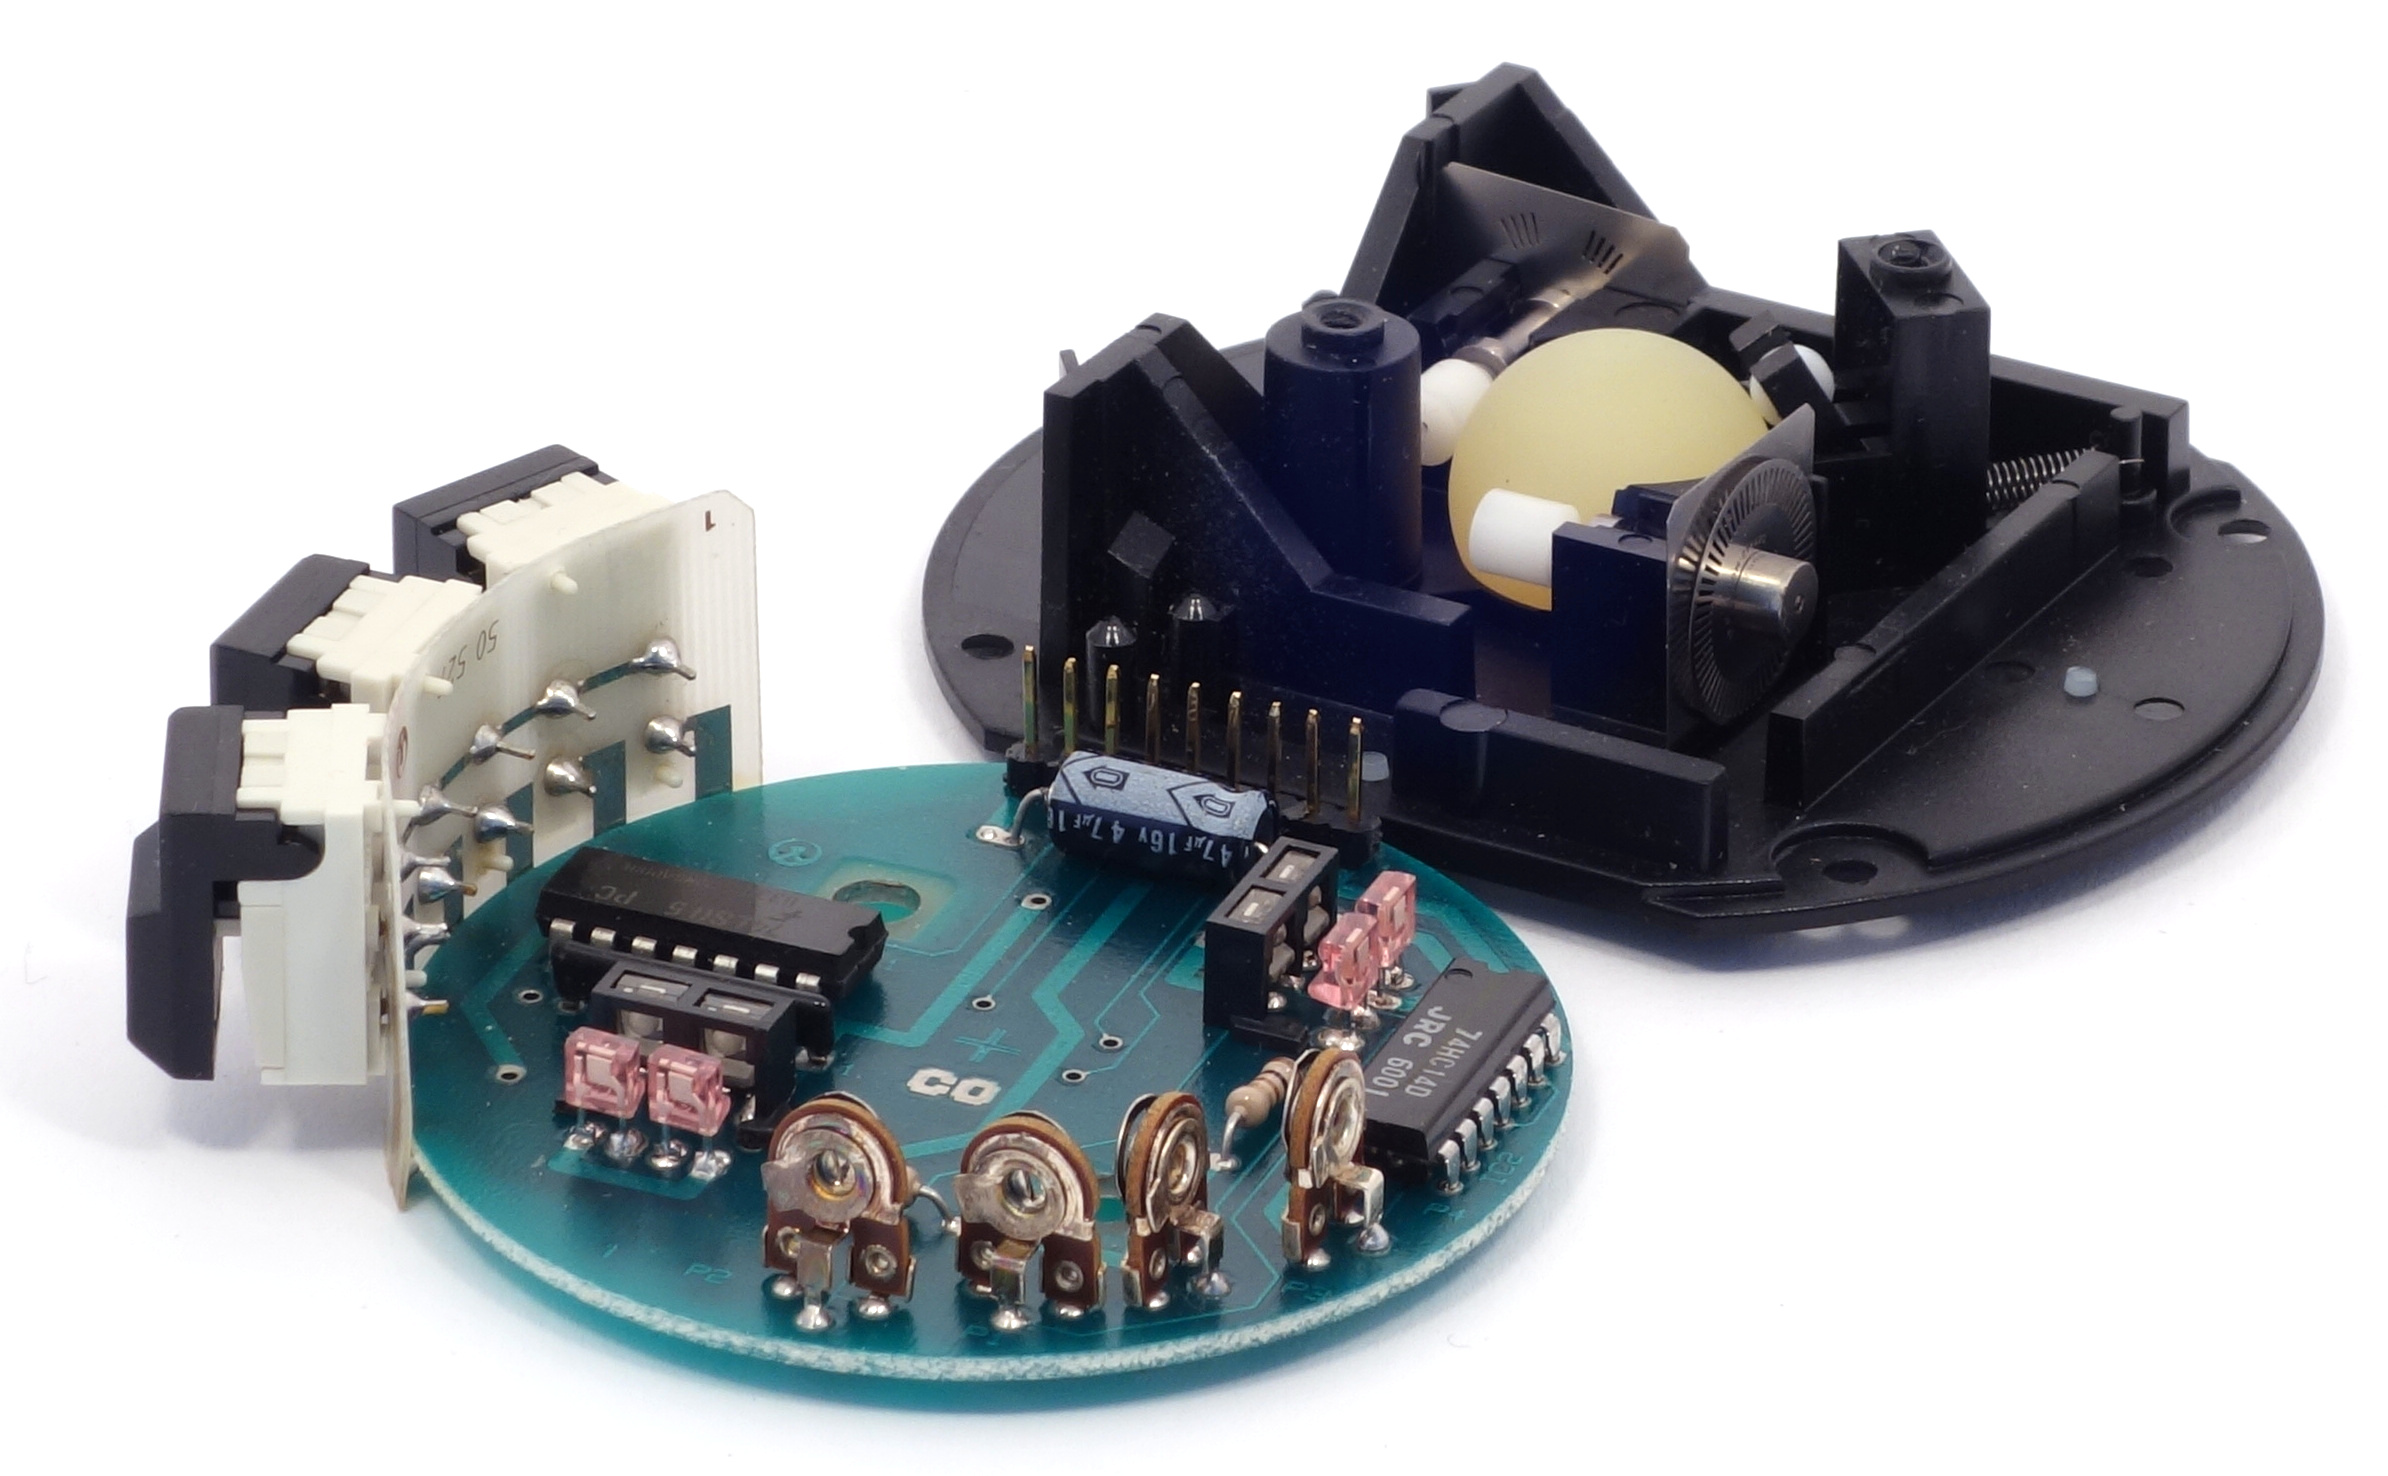
\includegraphics[scale=0.7]{1982_depraz_digimouse/inside_60.jpg}
    \caption{DIGIMOUSE P4 в разобранном виде}
    \label{fig:DIGIMOUSEP4Inside}
\end{figure}

Внутреннее устройство мыши показано на рис. \ref{fig:DIGIMOUSEP4Inside}. В мыши использованы оптомеханические энкодеры. Оптопары похожи на соответствующие детали в мышах 90-х годов, однако диск оптического прерывателя выполнен из металла и дополнительно оснащен неподвижной маской, уменьшающей площадь засветки. В процессе производства Logitech изначальная конструкция Dépraz Mouse претерпевала некоторые изменения: в частности, был заменен на пластмассу материал покрытия роликов и изначально металлического шара \cite{oldmouse}.

Наиболее активные продажи данной мыши приходятся на период с 1982 по 1984 годы (производство прекратилось в середине 80-х годов с выходом чрезвычайно популярной модели Logitech C7), а первоначальная розничная цена составляла 295 долларов. По ряду признаков Dépraz Mouse была существенно более технологически-совершенным устройством по сравнению с другими мышами первой половины 1980-х годов. Сочетание технологического превосходства, достаточно высокой цены и хорошей эргономики сделали данный манипулятор легендарным. В результате такой популярности, в первой половине 1990-х годов история <<куполообразной мыши>> неожиданно продолжилась с выпуском двух клонов P4: почти полная визуальная копия Hit Mouse производства Sunnyline \cite{sunnyline}, а также прозрачная Crystal Clear Mouse производства Suncom \cite{suncom}.

Как можно видеть (рис. \ref{fig:HitMousePic}), Hit Mouse максимально близко копирует внешний вид P4. Данная мышь предназначалась для компьютеров Amiga. Фактически, наиболее заметным изменением по сравнению с DIGIMOUSE является использование съемного поворотного кольца на защелках, позволяющего извлечь шар для удаления собравшегося мусора и чистки роликов (в P4 кольцо требовалось отвинчивать с помощью отвертки).

\begin{figure}[h]
   \centering
    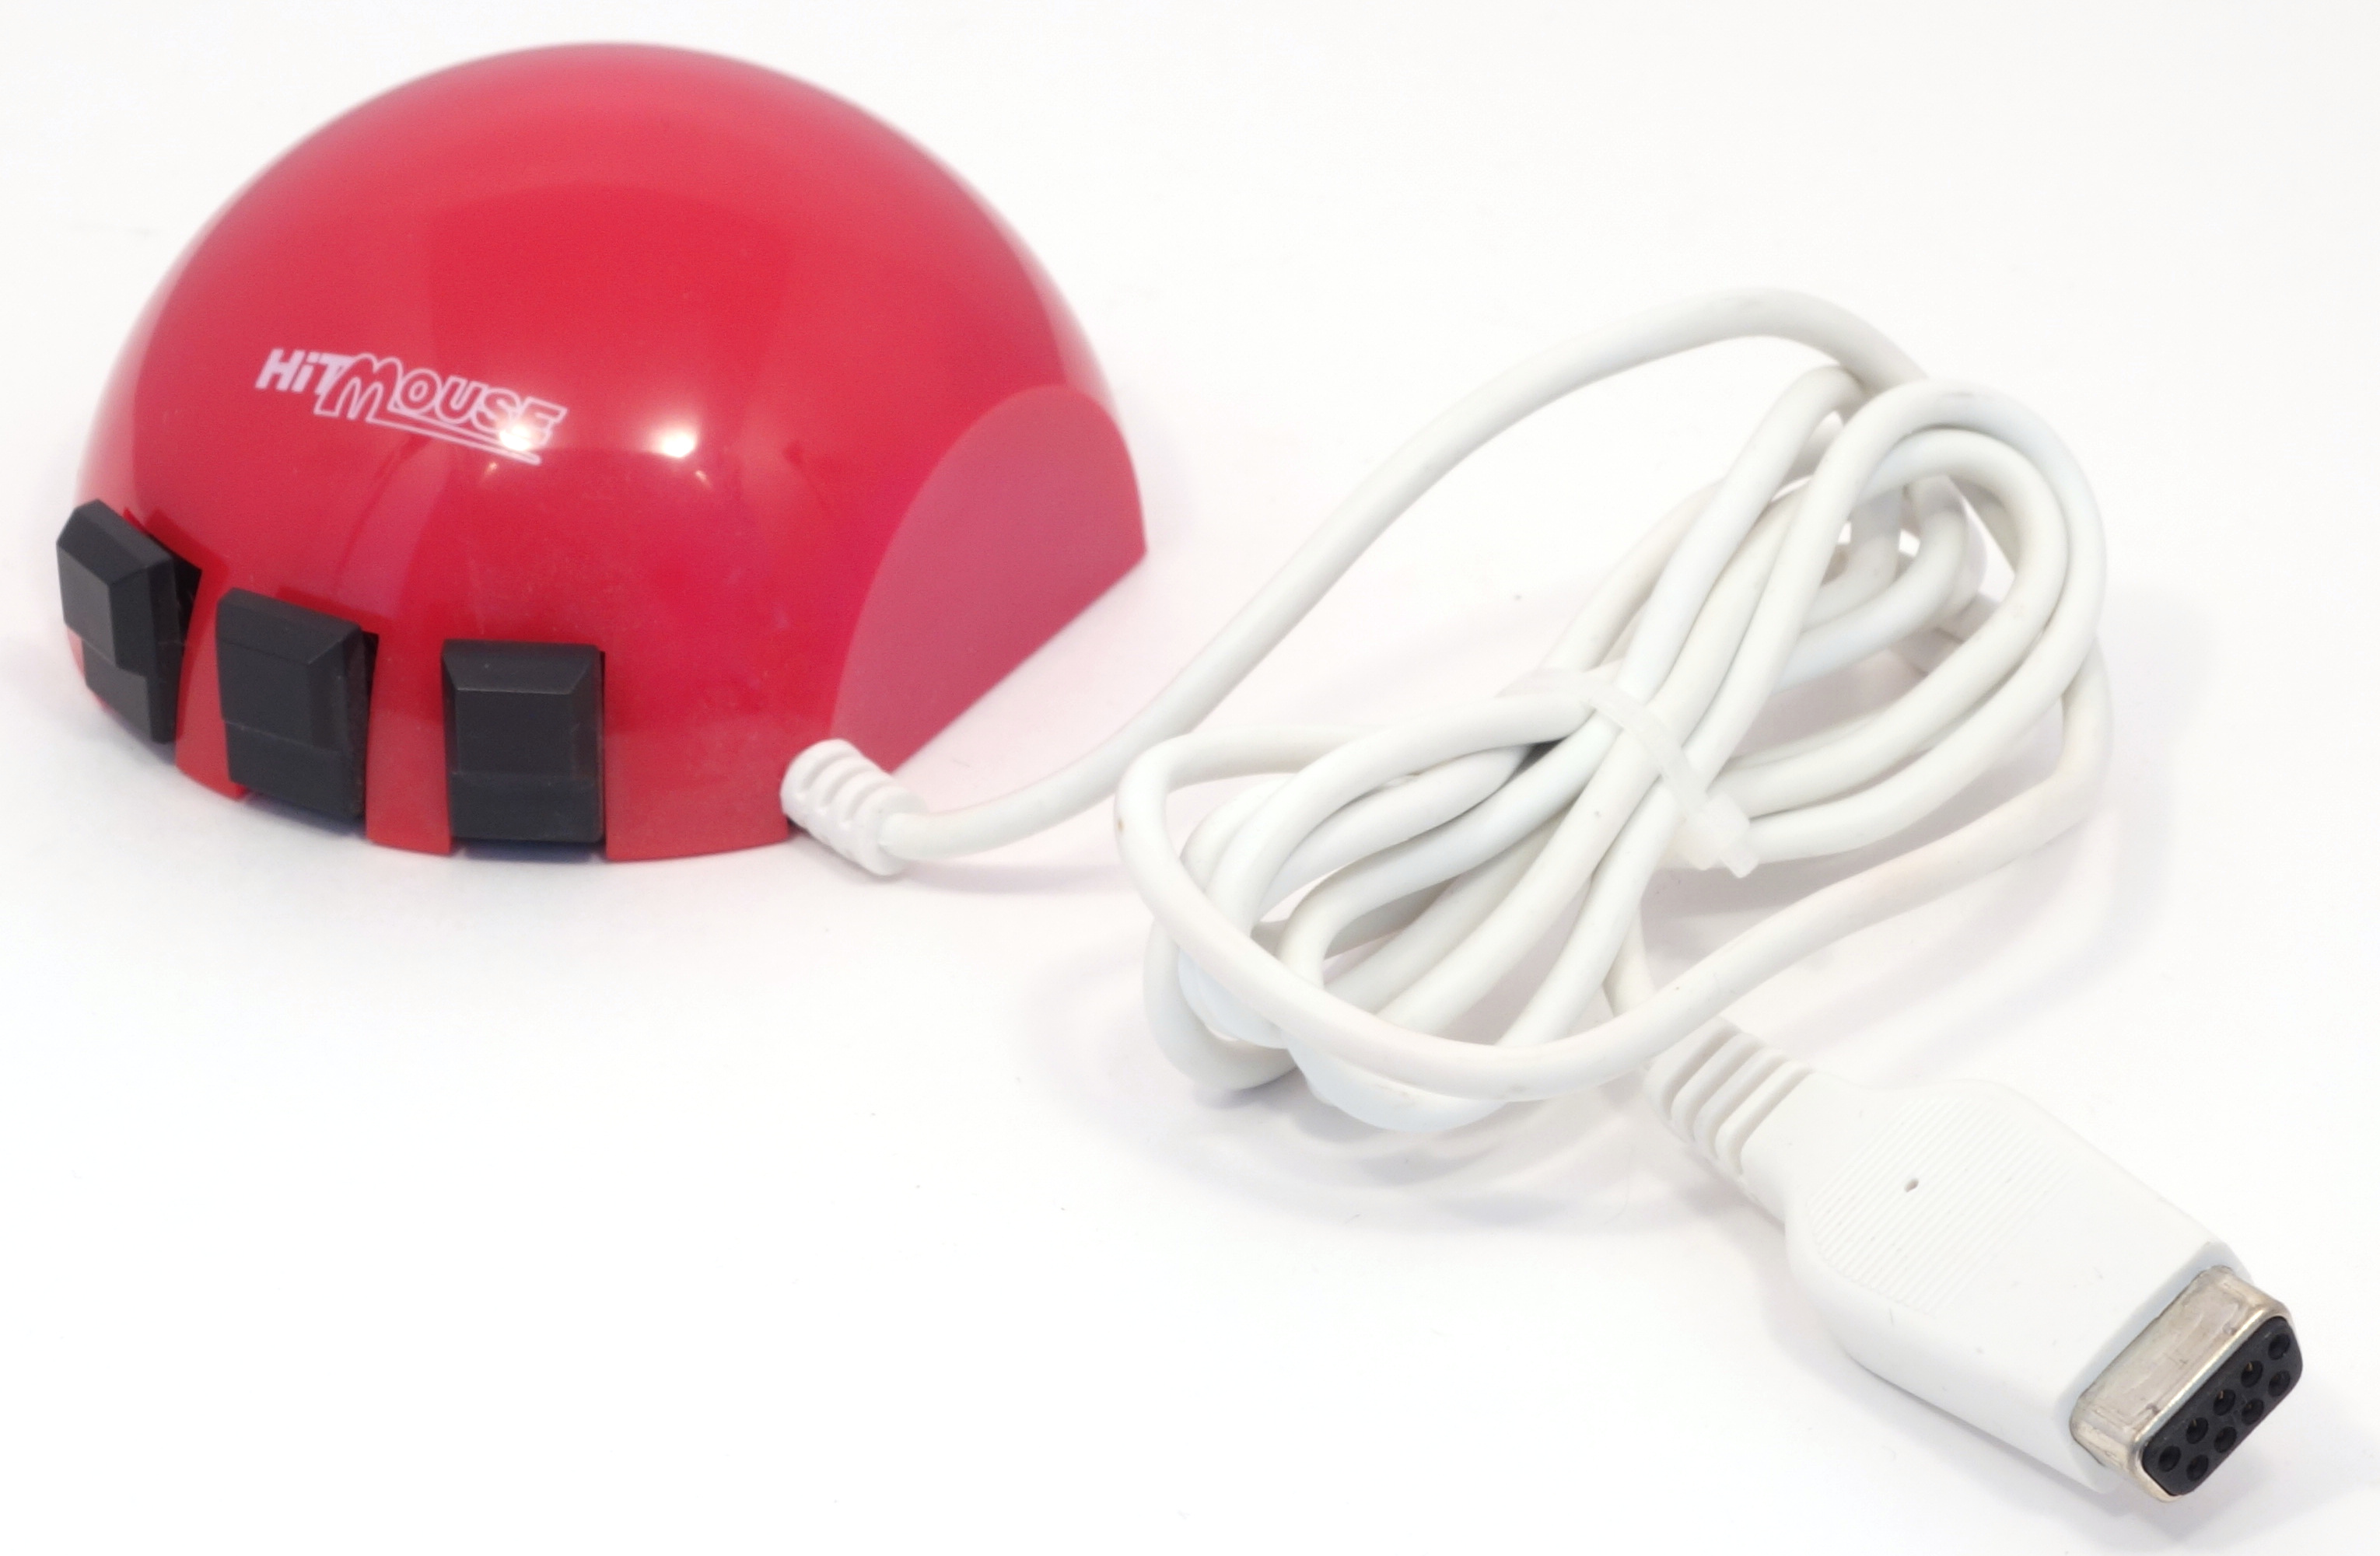
\includegraphics[scale=0.5]{1982_depraz_digimouse/hitmouse_pic_30.jpg}
    \caption{Sunnyline Hit Mouse}
    \label{fig:HitMousePic}
\end{figure}

Безусловно, копирование касалось только внешнего вида (наиболее распространенным был вариант с красным корпусом и черными кнопками, хотя \cite{sunnyline} упоминает также прозрачную версию). По внутреннему устройству Hit Mouse приближается к типичным оптомеханическим мышам середины 90-х годов (рис. \ref{fig:HitMouseInside}). C учетом того, что Hit Mouse выпускалась в 1991--1992 годах, в техническом плане ее можно считать вполне актуальным устройством для своего времени.

Однако, куполообразная форма, оказавшаяся чрезвычайно удачным решением на фоне других мышей 80-х годов, уже не вызывала такого энтузиазма у пользователей 90-х. В кратком обзоре, приведенном в Amiga Kickstart ее дизайн охарактеризован как очень необычный, требующий времени для того, чтобы к нему привыкнуть \cite{sunnyline}.

 \begin{figure}[h]
    \centering
    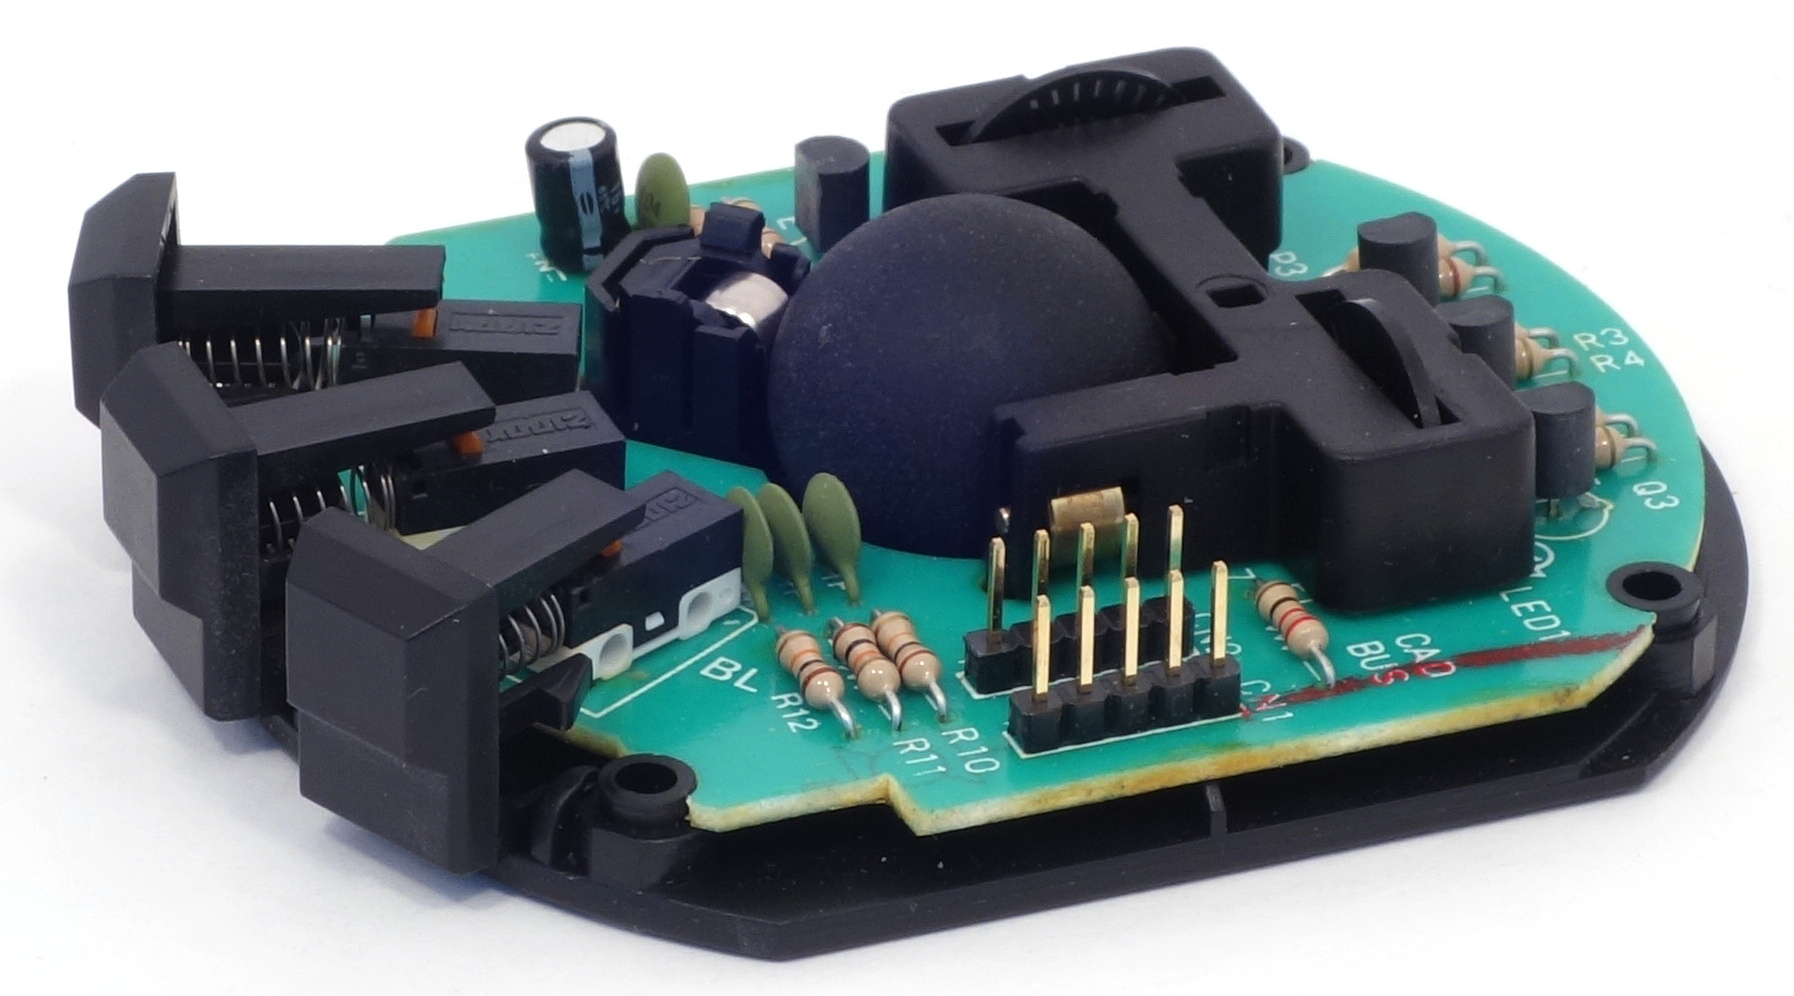
\includegraphics[scale=0.7]{1982_depraz_digimouse/hitmouse_inside_30.jpg}
    \caption{Sunnyline Hit Mouse в разобранном виде}
    \label{fig:HitMouseInside}
\end{figure}

\begin{thebibliography}{9}
\bibitem {DIGIMOUSE} J. Taylor. Faster then a speeding cursor key. // PC Magazine, V. 3, No. 2, February 7, 1984. "--- p. 243-245 \url{https://archive.org/details/PC-Mag-1984-02-07/page/n243/mode/2up}
\bibitem {oldmouse} Dépraz / Digimouse mouse $\sim$ oldmouse.com \url{https://web.archive.org/web/20211019061819/https://www.oldmouse.com/mouse/logitech/digimouse.shtml}
\bibitem {sunnyline} A. Kramer. PIEP-SHOW. M\"ause im Vergleich. Hit-Mouse II // Amiga Kickstart No. 10, Oktober, 1991. "--- p. 52-54 \url{https://archive.org/details/amiga-kickstart-91-10/page/52/mode/2up}
\bibitem {suncom} Crystal mouse, Suncom Technologies, 1991, USA. Mice Farm on Instagram. \url{https://www.instagram.com/p/CXYkzSpoqnL/}
\end{thebibliography}
\end{document}
